\graphicspath{ {./imagens/} }

\section{Descrição do Problema}
Considere o modelo cinemático de um uniciclo, dado por:
    \begin{align*}
            \dot{x} &= v_t cos(\theta)\\
            \dot{y} &= v_t sin(\theta)\\
            \dot{\theta} &= \omega
    \end{align*}

Em que $x$, $y$ e $\theta$ representam a posição em x, posição em y e orientação do veículo, enquanto
que $v_t$ e $\omega$representam as velocidades de translação e angular do veículo.

\section{Descrição da solução proposta}

Este trabalho propõe uma forma de se controlar o sistema para que ele siga uma referência de posição desejada utilizando linguagem natural. A referência utilizada é um outro carrinho hipotético que pode ser controlado manualmente ou programado para realizar certos movimentos pré-definidos dentro de uma área especifica. O ambiente de simulação foi provido pelo professor no ambiente moodle e abaixo pode-se observar uma figura que demonstra a aparência do simulador utilizado. O carrinho bege é a nossa referência enquanto o carrinho amarelo é o nosso carrinho a ser controlado.

\begin{figure}[H] 
    \centering
    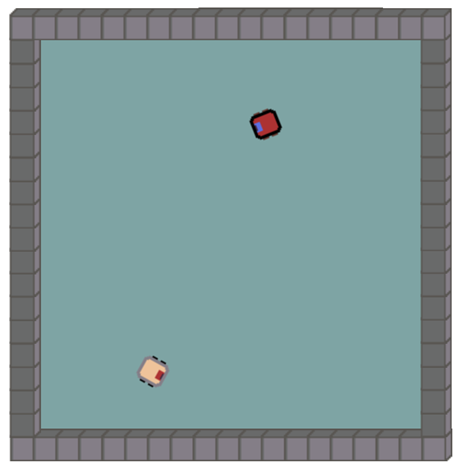
\includegraphics[scale=0.5]{carrinho_base.png}
    \caption{Ambiente de simulação}
\end{figure}

O controlador implementado foi baseado na técnica de controladores fuzzy utilizando
o método de inferência por regras de Mamdani. 
Inicialmente, para o projeto do controlador, identificou-se as entradas e saídas do controlador. As entradas são o erro do ângulo em relação a referência (e$\theta$) e o erro de posição do carrinho (Exy). 

\begin{figure}[H] 
    \centering
    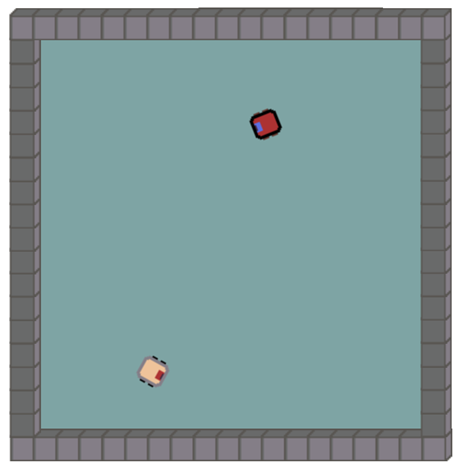
\includegraphics[scale=0.5]{carrinho_base.png}
    \caption{Ambiente de simulação}
\end{figure}

\section{Projeto do controlador fuzzy do robô}
    \subsection{Variáveis Linguísticas}
        \begin{itemize}
            \item{\bf{Antecedentes}}
                \begin{itemize}
                    \item Erro de ângulo
                    \item Erro de posição
                \end{itemize}
            \item{\bf{Saídas}}
                \begin{itemize}
                        \item Velocidade angular
                        \item Velocidade
                \end{itemize}
        \end{itemize}
    \subsection{Funções de pertinência}
    \begin{itemize}
        \item{\bf{Erro de ângulo}}
            \begin{itemize}
                \item Universo de discurso: $[-\pi,\pi]$
                \item Formato das funções de pertinência: Trapezoidal
                \item Número de conjuntos nebulosos: 5
            \end{itemize}  
            
            \begin{table}[H]
                \centering
                \begin{tabular}{|c|c|c|c|c|}
                    \hline
                    Conjunto               & Esq   & C\_Esq & C\_Dir & Dir \\ \hline
                    Erro Negativo Grande   & -5    & -5    & -2.5  & -2    \\
                    Erro Negativo Pequeno  & -3    & -2    & -1    & 0     \\
                    Erro  Nulo             & -1    & -0.5  & 0.5   & 1     \\
                    Erro Positivo Pequeno  & 0     & 1     & 2     & 3     \\
                    Erro Positivo Grande   & 2     & 2.5   & 5     & 5     \\ \hline
                \end{tabular}
                \caption{Erro de ângulo}
            \end{table}

            \begin{figure}[H] 
                \centering
                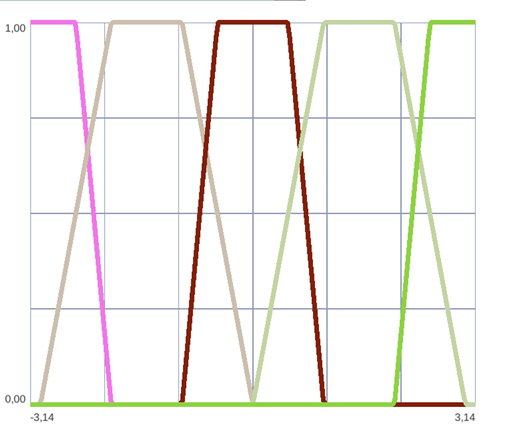
\includegraphics[scale=0.7]{in_angulo.png}
                \caption{Erro de ângulo}
            \end{figure}
            
            \newpage    
        
        \item{\bf{Erro de posição}}
            \begin{itemize}
                \item Universo de discurso: $[-10,10]$
                \item Formato das funções de pertinência: Trapezoidal
                \item Número de conjuntos nebulosos: 5
            \end{itemize}

            \begin{table}[H]
                \centering
                \begin{tabular}{|c|c|c|c|c|}
                    \hline
                    Conjunto               & Esq   & C\_Esq & C\_Dir & Dir \\ \hline
                    Erro Negativo Grande   & -10   & -10   & -2.5  & -2    \\
                    Erro Negativo Pequeno  & -3    & -2    & -1    & 0     \\
                    Erro  Nulo             & -1    & -0.5  & 0.5   & 1     \\
                    Erro Positivo Pequeno  & 0     & 1     & 2     & 3     \\
                    Erro Positivo Grande   & 2     & 2.5   & 10    & 10    \\ \hline
                \end{tabular}
                \caption{Erro de posição}
            \end{table}

            \begin{figure}[H] 
                \centering
                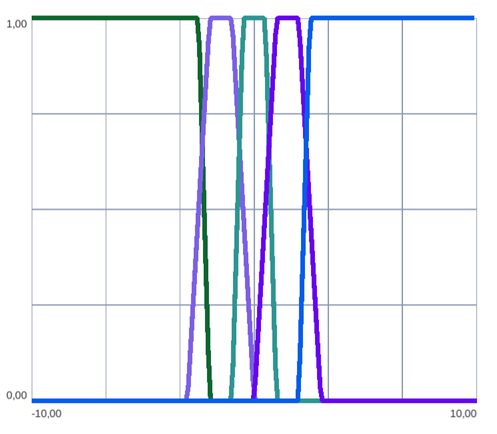
\includegraphics[scale=0.7]{imagens/in_posicao.png}
                \caption{Erro de posição}
            \end{figure}

            \newpage
            
        \item{\bf{Velocidade angular}}
            \begin{itemize}
                \item Universo de discurso: $[-5,5]$
                \item Formato das funções de pertinência: Trapezoidal
                \item Número de conjuntos nebulosos: 5
            \end{itemize}

            \begin{table}[H]
                \centering
                \begin{tabular}{|c|c|c|c|c|}
                    \hline
                    Conjunto               & Esq   & C\_Esq & C\_Dir & Dir   \\ \hline
                    Gira Muito a Esq       & -5    & -5     & -2.5   & -2    \\
                    Gira Pouco a Esq       & -3    & -2     & -1     & 0     \\
                    Não Gira               & -1    & -0.5   & 0.5    & 1     \\
                    Gira Pouco a Dir       & 0     & 1      & 2      & 3     \\
                    Erro Muito a Dir       & 2     & 2.5    & 5      & 5     \\ \hline
                \end{tabular}
                \caption{Velocidade angular}
            \end{table}

            \begin{figure}[H] 
                \centering
                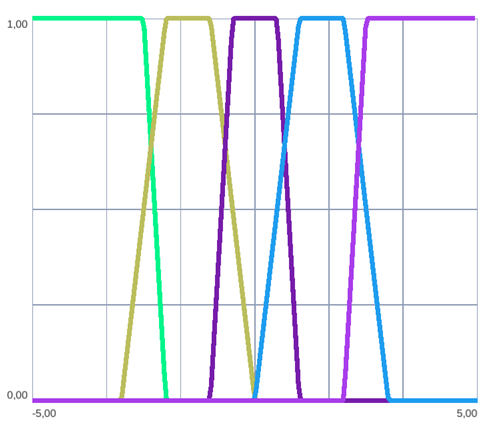
\includegraphics[scale=0.7]{imagens/out_velocidadeang.png}
                \caption{Velocidade angular}
            \end{figure}

            \newpage
            
        \item{\bf{Velocidade}}
            \begin{itemize}
                \item Universo de discurso: $[-5,5]$
                \item Formato das funções de pertinência: Trapezoidal
                \item Número de conjuntos nebulosos: 5
            \end{itemize}

            \begin{table}[H]
                \centering
                \begin{tabular}{|c|c|c|c|c|}
                    \hline
                    Conjunto               & Esq   & C\_Esq & C\_Dir & Dir   \\ \hline
                    Freia Muito            & -5    & -5     & -2.5   & -2    \\
                    Freia Pouco            & -3    & -2     & -1     & 0     \\
                    Nem Acel e Nem Freia   & -1    & -0.5   & 0.5    & 1     \\
                    Acelera Pouco          & 0     & 1      & 2      & 3     \\
                    Acelera Muito          & 2     & 2.5    & 5      & 5     \\ \hline
                \end{tabular}
                \caption{Velocidade}
            \end{table}

            \begin{figure}[H] 
                \centering
                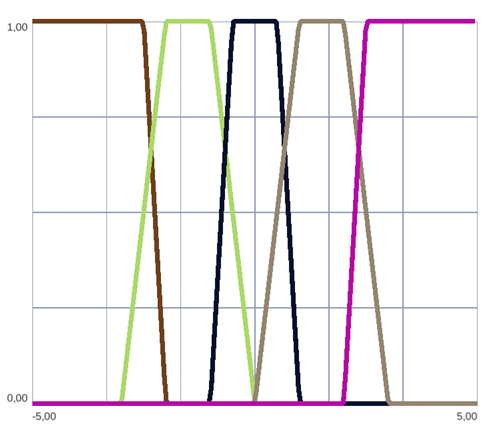
\includegraphics[scale=0.7]{imagens/out_velocidade.png}
                \caption{Velocidade}
            \end{figure}

            \newpage
    \end{itemize}
    
    \subsection{Base de Regras FUZZY}

